\section{Fixed-Weight Replay and Online State-Boundary Results}\label{sec:r42-r44-verified}

This section gives the measurements behind the paper's receiver, state and
attacker/workload boundaries. The fixed-weight replay and the online planner
stress test are separate studies. The former measures a passive receiver on
saved model output sent through a timed TLS loopback; the latter invokes a
served planner and simulated user in a native retail sandbox. The sandbox
study does not measure WRA's privacy protection.

\subsection{Local model generation and timed TLS replay}
Three pinned local weight artifacts generated five templates for each of 100 synthetic topics (1,500 outputs), with a 128-token output budget. The primary binary target is medical versus nonmedical category, with 50 topics per class. Each of five test folds contains ten topics of each class and all their templates; chance BA is 50\%. The secondary task predicts 100 known topic labels with one template held out per fold; chance BA is 1\%. This second task is not new-topic generalization. Saved native chunks are replayed through timed TLS loopback. Attackers observe response application-record lengths and timing; content, requests and handshakes are excluded. No cloud-service, WAN, real-user-topic or online defended-generation outcome is measured.

For each defended test view, D0 learns on clean training data and D2 on defended training data. The matched-three comparison separately takes the highest OOF BA among logistic regression, random forest and gradient boosting on the same five folds used for reporting. This non-nested winner selection can be optimistic. Full12 (primary) and Full9 (secondary) add the declared attacks; their suite maxima are exploratory, not unbiased performance estimates. Bootstrap intervals resample the finite topic inventory and recompute maxima over saved predictions, without refitting attacks or recalibrating the defense. This does not remove winner-selection bias.

The Qwen~8B base-origin raw matched-three reference is 79.0\% BA. At local batch point 1 (four native chunks per batch), matched D0 and D2 are 50.0\% and 73.2\%. These three values use the same prespecified learner classes with separate winner selection in each condition, not a paired effect estimate or interval for one fixed classifier. Full12 is 73.4\% and must not be substituted for the matched D2 value. D0 logistic regression has AUROC 0.678272 despite BA 50.0\%, so the thresholded chance result does not show zero information. On the same 500 replays over 100 topics, response application TLS bytes are 470,239 versus 1,234,823 paired raw bytes (0.380815$\times$). Paired session completion differences have median $+0.1524$~ms and 95th percentile $+2.3814$~ms; original content-chunk endpoint delays have median $+27.5909$~ms and 95th percentile $+65.7301$~ms. Aggregation reduces framing/record overhead; the ratio is not total request traffic. The full costs for both 81-row grids are printed in \S\ref{sec:r46-e4-costs} with their own raw origins.

At the default source comparisons, all 45 source--target--fold combinations share the same 32-byte bucket quantum, four-chunk batching parameter, or 32-byte cell/50-ms tick parameters. Batching is source-independent by design; source-training quantiles for buckets and cells round to identical values. Their zero imported-minus-local differences are identical-parameter controls and provide no evidence of calibration transfer. Some primary hard-cap source/fold comparisons differ, but Qwen~8B and Qwen~0.6B both use 87 events in fold IDs 1 and 3 and differ only in the other three folds; Llama~1B uses 128 in every fold. The six primary contrasts are listed in Table~\ref{tab:r46-hardcap-conditional}. Intervals condition on fitted attackers and omit recalibration/refitting uncertainty. Secondary fixed-observed-winner sign-flip tests assume sign symmetry or exchangeability and do not correct winner selection. Holm adjustment covers two imported-source comparisons per target only; it is not global across targets, controls and points. The reported analysis lacks a local fitting-variability control to distinguish a source effect from finite-training-sample calibration variation.

The original 35,000-session queue stopped with 34,440 completed sessions and one started session without a saved outcome. That outcome remains unknown. A separate continuation collected the 559 original jobs that had not started and a complete 500-session repetition of the affected Qwen~8B constant-rate arm. The repeat was selected after the interruption. It uses separate session identities and a new local TLS runtime/batch; the collector still calls the original local TLS implementation. Four overlapping continuation jobs are retained separately. Of 600 planned fold evaluations, ten affected folds use the whole repeated arm; the others use original completed captures or independently collected never-started jobs. Reconstruction of 35,000 routed captures and 600 evaluations does not make the original run complete or retrain the classifiers.

For the 495 old/new matched sessions, response bytes and application-record counts agree in every pair. The median across topic means of receiver completion differences is $-0.461$~ms; their empirical 5th--95th percentile range is $[-1.398,0.185]$~ms. This describes observed timing differences, not a confidence interval, exchangeability test or proof that batch effects vanished. The proxy-to-direct path and concurrency changes in the following online study belong to R44, not E4. All original outcomes, repeats and continuation identities remain preserved.

\begin{table*}[t]\centering\fontsize{8}{9.5}\selectfont
\setlength{\tabcolsep}{3pt}
\caption{Post-interruption recovery. Four controls, held-out-topic binary. Cells: Full12 BA and frozen paired imported-minus-local percentage-point difference. Source rows/target columns; local identity diagonal. Bucket, batch and fixed-cell defaults have identical parameters across sources; their zero differences do not test transfer. Complete absolute/paired intervals and all contrasts retained in accompanying tables/CSV/JSON. Qwen 8B fixed-cell point 2 uses a separately repeated arm; the original session is missing.}
\begin{tabular}{lllll}\toprule
Control & Source calibration & qwen3:8b & qwen3:0.6b & llama3.2:1b\\\midrule
Buckets & qwen3:8b & 58.6 (local) & 58.4 (+0.0) & 60.4 (+0.0)\\
Buckets & qwen3:0.6b & 58.6 (+0.0) & 58.4 (local) & 60.4 (+0.0)\\
Buckets & llama3.2:1b & 58.6 (+0.0) & 58.4 (+0.0) & 60.4 (local)\\
\midrule
Chunk batches & qwen3:8b & 73.4 (local) & 73.2 (+0.0) & 71.8 (+0.0)\\
Chunk batches & qwen3:0.6b & 73.4 (+0.0) & 73.2 (local) & 71.8 (+0.0)\\
Chunk batches & llama3.2:1b & 73.4 (+0.0) & 73.2 (+0.0) & 71.8 (local)\\
\midrule
Fixed cells* & qwen3:8b & 57.2 (local) & 58.4 (+0.0) & 60.8 (+0.0)\\
Fixed cells* & qwen3:0.6b & 57.2 (+0.0) & 58.4 (local) & 60.8 (+0.0)\\
Fixed cells* & llama3.2:1b & 57.2 (+0.0) & 58.4 (+0.0) & 60.8 (local)\\
\midrule
True hard cap & qwen3:8b & 76.0 (local) & 72.6 (+0.6) & 69.4 (+0.2)\\
True hard cap & qwen3:0.6b & 74.8 (-1.2) & 72.0 (local) & 70.2 (+1.0)\\
True hard cap & llama3.2:1b & 79.4 (+3.4) & 75.8 (+3.8) & 69.2 (local)\\
\bottomrule\end{tabular}
\end{table*}

\begin{table*}[t]\centering\fontsize{8}{9.5}\selectfont
\setlength{\tabcolsep}{3pt}
\caption{Post-interruption recovery. Four controls, known-topic, held-out-template100way. Cells: Full9 BA and frozen paired imported-minus-local percentage-point difference. Source rows/target columns; local identity diagonal. Bucket, batch and fixed-cell defaults have identical parameters across sources; their zero differences do not test transfer. Complete absolute/paired intervals and all contrasts retained in accompanying tables/CSV/JSON. Qwen 8B fixed-cell point 2 uses a separately repeated arm; the original session is missing.}
\begin{tabular}{lllll}\toprule
Control & Source calibration & qwen3:8b & qwen3:0.6b & llama3.2:1b\\\midrule
Buckets & qwen3:8b & 2.4 (local) & 1.8 (+0.0) & 1.6 (+0.0)\\
Buckets & qwen3:0.6b & 2.4 (+0.0) & 1.8 (local) & 1.6 (+0.0)\\
Buckets & llama3.2:1b & 2.4 (+0.0) & 1.8 (+0.0) & 1.6 (local)\\
\midrule
Chunk batches & qwen3:8b & 14.0 (local) & 9.4 (+0.0) & 7.8 (+0.0)\\
Chunk batches & qwen3:0.6b & 14.0 (+0.0) & 9.4 (local) & 7.8 (+0.0)\\
Chunk batches & llama3.2:1b & 14.0 (+0.0) & 9.4 (+0.0) & 7.8 (local)\\
\midrule
Fixed cells* & qwen3:8b & 1.6 (local) & 2.0 (+0.0) & 1.8 (+0.0)\\
Fixed cells* & qwen3:0.6b & 1.6 (+0.0) & 2.0 (local) & 1.8 (+0.0)\\
Fixed cells* & llama3.2:1b & 1.6 (+0.0) & 2.0 (+0.0) & 1.8 (local)\\
\midrule
True hard cap & qwen3:8b & 68.4 (local) & 50.4 (+1.0) & 35.4 (+1.6)\\
True hard cap & qwen3:0.6b & 66.8 (-1.6) & 49.4 (local) & 34.0 (+0.2)\\
True hard cap & llama3.2:1b & 67.8 (-0.6) & 46.8 (-2.6) & 33.8 (local)\\
\bottomrule\end{tabular}
\end{table*}

\begin{table*}[t]\centering\footnotesize
\caption{All six default hard-cap imported-minus-local primary contrasts. Differences and 95\% topic-bootstrap intervals are in BA percentage points, conditional on fitted attackers. The secondary fixed-winner sign-flip $p_{\mathrm H}$ adjusts only the two imports per target; it omits refitting and winner-selection uncertainty. No local fitting-variability control is reported.}\label{tab:r46-hardcap-conditional}
\begin{tabular}{llrrr}\toprule
Imported source & Target & Difference & Conditional 95\% interval & $p_{\mathrm H}$\\\midrule
Qwen 0.6B & Qwen 8B & $-1.2$ & $[-2.6,1.2]$ & 0.2378\\
Llama 1B & Qwen 8B & $+3.4$ & $[0.8,5.4]$ & 0.0112\\
Qwen 8B & Qwen 0.6B & $+0.6$ & $[-2.4,1.8]$ & 0.8122\\
Llama 1B & Qwen 0.6B & $+3.8$ & $[0.0,6.0]$ & 0.1224\\
Qwen 8B & Llama 1B & $+0.2$ & $[-3.0,4.4]$ & 1.0000\\
Qwen 0.6B & Llama 1B & $+1.0$ & $[-2.2,4.8]$ & 1.0000\\
\bottomrule\end{tabular}
\end{table*}

\begin{figure*}[t]
  \centering
  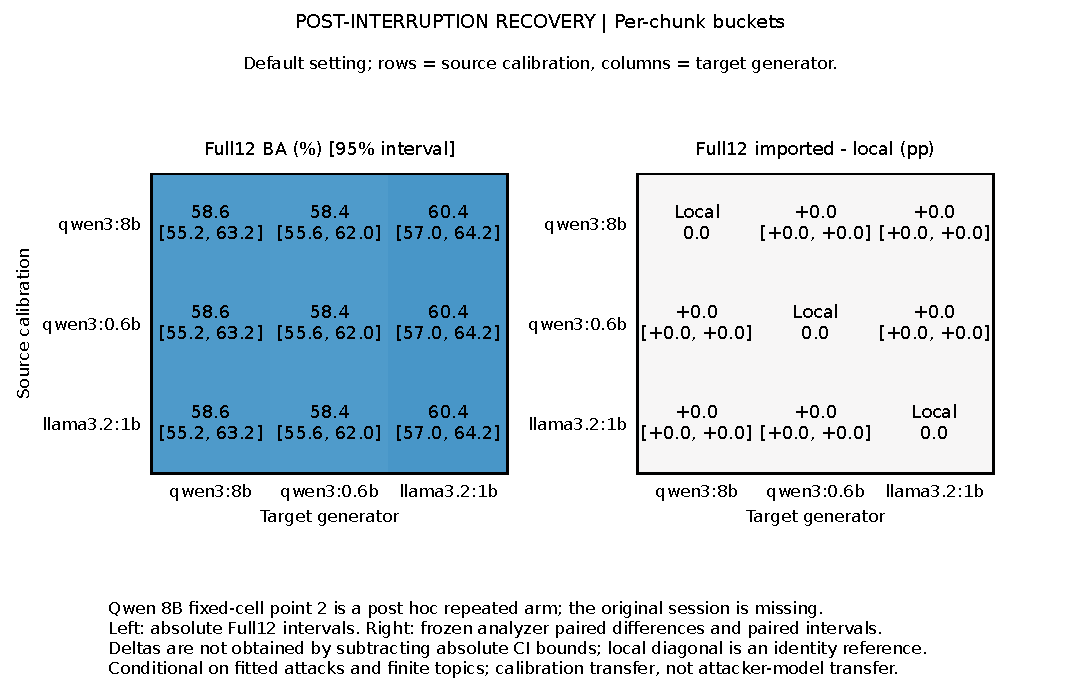
\includegraphics[width=0.96\textwidth]{figures/r42-e4-primary-bucket-verified.pdf}
  \caption{Archived default bucket matrix from the post-interruption replay projection. All source folds use the same 32-byte quantum: the zero differences compare identical parameters and do not measure transfer. The figure's historical calibration-transfer label denotes the comparison layout, not evidence of portability. Conditional intervals and repeated-arm provenance retain their stated limitations.}
  \label{fig:r42-e4-supp-verified}
\end{figure*}

\subsection{Online planner: nonrandom replacement cohort}
The original served GLM run stopped after 347 of 900 planned episodes because
of transport failures. At interruption, 113 task--repeat blocks had all
three arms; the other 187 blocks were selected using terminal-file existence,
not measured utility. The complete blocks and all eight additional GLM
terminal episodes remain in the artifact. For each of the 187 incomplete
blocks, a new \texttt{qwen3.8-flash-next} planner and simulated user were run
in all three arms on independently cloned states: no cover, one extra read,
and one same-ID item write. This gives 561 fresh episodes from 98 tasks and
46 customers. The served model name is an alias; fixed model weights are not
claimed. The interrupted selection is nonrandom, and comparisons are within
this model and cohort; no arm is paired across model services.

The read or write is triggered at most once immediately after the first
planner-originated order-details lookup, and its reply is not delivered to the
planner. A valid candidate is chosen from the initial fixture without reading
the task's reference actions. Of 187 episodes per cover arm, the extra tool
executed in 97 and was not exposed in 90. The write arm recorded 97 write
attempts and 97 state effects, each consuming the native pending-item
modification eligibility. All unexposed episodes remain in the denominator.
The write is a controlled state/utility stress condition, not a claim of a
deployed privacy defense or discovered authorization bypass.

The generated table reports raw success counts out of 187 separately from
task-weighted means: 29 tasks contribute one selected repetition, 49 contribute
two and 20 contribute three. For each contrast, selected repetitions are first
averaged within task, and the 98 task means are then equally weighted. The
predeclared task-cluster bootstrap and sign-flip use 20,000 draws; Holm covers
the two displayed paired tests. A customer-cluster sensitivity retains tasks
within each of 46 customers. Its 95\% intervals for read minus no cover and
write minus no cover are $[-3.65,4.74]$ and $[-61.39,-32.04]$ percentage
points, respectively; the corresponding Holm-adjusted sign-flip values are
0.8211 and $9.9995\times10^{-5}$. The intervals describe this nonrandom
cohort; the sign-flip tests additionally require sign symmetry or
exchangeability. They do not establish equivalence of read and no cover.

\begin{table*}[t]\centering\footnotesize
\caption{R44 verified three-arm utility. Each arm has 187 episodes from 98 tasks; the selected blocks are nonrandom. Task-weighted success, paired difference, and intervals weight each task equally after averaging its available repeats. The paired tests assume task-level sign symmetry; Holm covers the two shown contrasts. This is a sandbox utility stress test.}
\begin{tabular}{lrrrr}\hline
Condition & Successes /187 & Task mean (\%) [95\%] & Difference (pp) [95\%] & Holm $p$\\\hline
No cover & 154/187 & 82.7 [75.5, 89.3] & -- & --\\
Read cover & 156/187 & 83.3 [76.5, 89.6] & +0.7 [-4.9, +6.1] & 0.859\\
Write cover & 72/187 & 35.7 [26.7, 45.1] & -46.9 [-56.8, -36.9] & $<0.001$\\
\hline\end{tabular}
\end{table*}


The verifier reconstructed all 561 saved conversations and 4,176 tool events;
9,801 model decisions were checked against and decoded from their saved
requests and provider receipts. No completed response was intentionally
resampled. Across no-cover, read-cover and write-cover arms respectively,
real planner tool calls were 1,319, 1,323 and 1,340, with 61, 52 and 90
recorded real-tool failures. Cover-tool failures were zero. Model request
attempts were 3,359, 3,353 and 3,206, including 35, 34 and 38 recorded
infrastructure failures. The 10 interrupted requests without a locally saved
response or error are preserved separately: their server-side completion and
waiting times are unknown and are not included in recorded transport-time
totals. Summed per-call waiting times overlap under concurrency, and cached
reconstruction can affect final-visit wall time; neither is a complete
end-to-end deployment cost.

The frozen inference request used a 16,384-token output budget, 600-second
timeout and default certificate verification. During collection, the target
domain was moved from the system-proxy path to a direct connection, and the
effective scheduling limit changed from ten to two concurrent workers. The
request body and source/configuration fingerprints stayed fixed. Both paths
passed task-free interface probes, but this does not locate the cause of the
earlier connection failures. These operational changes and the unknown waits
limit cross-run latency and cost comparisons.

The 113 completed GLM blocks are retained as a separate, post-interruption
exploratory description over 80 tasks. Their success counts were 83, 87 and
28 out of 113 for no cover, read cover and write cover. Equal-task-weighted
paired differences were $+3.1$ percentage points for read and $-45.6$ for
write, with task-cluster 95\% intervals $[-6.5,12.7]$ and $[-57.9,-32.7]$,
respectively. These completed-before-interruption blocks are not a random
sample, are not paired with Qwen arms, and are not an independent test of
privacy protection. The eight additional terminal GLM episodes are preserved
but do not form complete three-arm blocks.

The artifact retains the respective protocols, saved decisions, interruption
and transport amendments, selection manifests, verification receipts,
prediction outputs and result projections under
\path{experiments/sp2027-r42-open-weights/additions/interrupted-recovery/},
\path{experiments/sp2027-r43-agent-utility/} and
\path{experiments/sp2027-r44-qwen-agent-utility/}. The Qwen statistics and
counts above are reconstructed from the verified 561-episode projection; the
GLM description is reconstructed from the verified 347-episode partial
receipt and 113-block projection. The archived records support separate
reconstruction rather than substituting one model's observations for the
other's.
